\section{Aufbau der Stoffe}

\subsection{Bindungsarten}
\begin{itemize}
	\item Kovalente Bindung (Atombindung)
		\begin{itemize}
			\item 2 nichtmetallische Atome
			\item Moleküle
		\end{itemize}
	\item Ionenbindung
		\begin{itemize}
			\item Elektrostatische Anziehung zwischen pos. und neg. geladenem Ion
			\item Salze
		\end{itemize}
	\item Metallbindung
		\begin{itemize}
			\item Elektrostatische Anzehung zwischen met. Kation und $e^-$
			\item Metalle und Legierungen
		\end{itemize}
\end{itemize}

\subsection{Stoffklassen}
\begin{itemize}
	\item Flüchtige Stoffe (molekulare Stoffe und Edelgase)
	\item Salzartige Stoffe
	\item Metallische Stoffe
	\item Hochmolekulare Stoffe (Polymere)
	\item Diamantartige Stoffe
\end{itemize}

\subsection{Kristallstrukturen}
\begin{itemize}
	\item Kristalline Feststoffe (regelmässige Anordnung = Fernordnung), z.B. Metalle, Salze, diamantartige
	\item Amorphe Feststoffe (unregelmässige Anordnung = Nahordnung), z.B. Kunststoffe, Glas
\end{itemize}

\subsection{Dichteste Kugelpackungen}
\begin{figure}[htbp]
	\begin{subfigure}{0.49\linewidth}
		\centering
		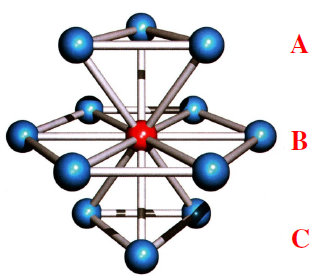
\includegraphics[width=0.49\linewidth]{images/1_kubisch_dichteste_KuPa.png}
		\caption{Kubisch dichteste Kugelpackung}
	\end{subfigure}
	\begin{subfigure}{0.49\linewidth}
		\centering
		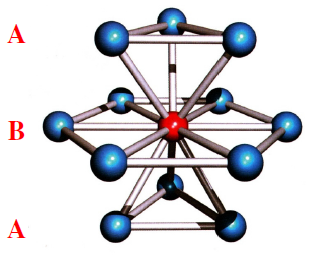
\includegraphics[width=0.49\linewidth]{images/1_hexagonal_dichteste_KuPa.png}
		\caption{Hexagonal dichteste Kugelpackung}
	\end{subfigure}
\end{figure}

\subsubsection{Lücken}
\begin{itemize}
	\item Oktaederlücken: oktaedrisch von 6 Atomen umgeben
	\item Tetraederlücken: tetraedrisch von 5 Atomen umgeben
	\item Koordinationszahl (KZ): Zahl der nächsten Nachbarteilchen
\end{itemize}

\subsection{Elementarzelle}
Kleinste Einheit einer Kristallstruktur. Erlaubt eindeutige Beschreibung des atomaren Aufbaus. \\

\begin{figure}[htbp]
	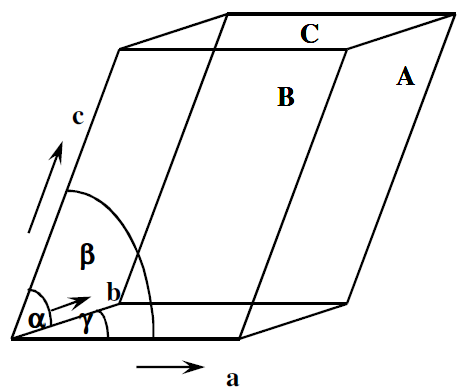
\includegraphics[width=3.5cm]{images/1_Elementarzelle.png}
\end{figure}
Durch 6 Gitterparameter $a,b,c,\alpha,\beta,\gamma$ eindeutig bestimmt. Es existieren 14 Arten von Elementarzellen: \\

\begin{figure}[htbp]
	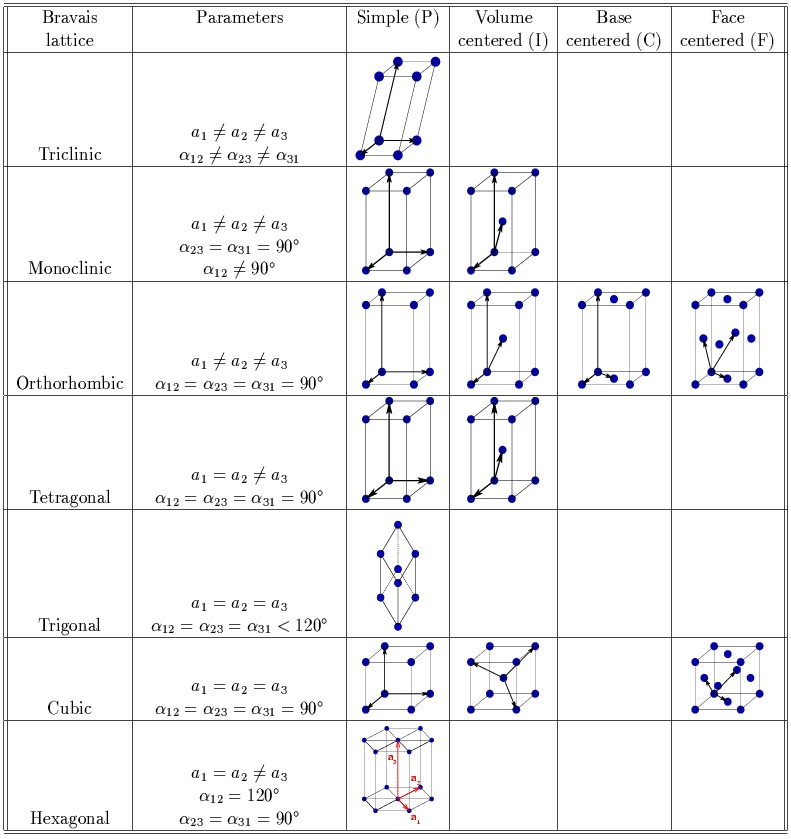
\includegraphics[width=\linewidth]{images/1_Kristallstrukturen.png}
\end{figure}


\subsection{Packungsdichte}
Packungsdichte $P = \frac{V_{Atome}}{V_{Elementarzelle}}$, macht Aussage zu Raumausnutzung.

\subsection{Gitterfehler}
\begin{itemize}
	\item Versetzung
	\item Unbesetzter Gitterplatz
	\item Fremdatom in Gitterlücke
	\item Fremdatom in Gitterplatz
\end{itemize}